% authored by Menelaus PERDIKEAS mperdikeas@gmail.com
\documentclass[9pt,twoside,openright,a4paper,pagesize]{report}

\usepackage{pslatex,palatino,avant,graphicx,color}
\usepackage[lmargin=4cm,rmargin=2cm,tmargin=3.5cm,bmargin=4.5cm,head=30pt,foot=60pt]{geometry}
\usepackage{comment}
\usepackage{datetime}
%TODO: understand why I can't change the date format
%\newdateformat{yyyymmdddate}{\THEYEAR\--\twodigit{\THEMONTH}\--\twodigit{\THEDAY}}
\usepackage[table,xcdraw]{xcolor}
\usepackage{fancyvrb}
\usepackage{multicol}
\setlength\columnsep{-8cm}
\usepackage{fancyhdr}
\usepackage{titling}
\usepackage{lastpage}
\usepackage{listings}
\usepackage{setspace}
\usepackage{enumitem}
\usepackage{rotating}
\usepackage{longtable}
\usepackage[htt]{hyphenat}
\usepackage[normalem]{ulem}
\usepackage[hyphens]{url}

\usepackage[table,xcdraw]{xcolor}
\usepackage{tikz}
\newcommand*\circled[1]{\tikz[baseline=(char.base)]{ 
            \node[shape=circle,fill=blue!20,draw,inner sep=2pt] (char) {#1};}}


\usepackage{titlesec}
\newcommand{\sectionbreak}{\clearpage}
\newcommand{\componentAlias}{}
\newcommand{\component}[2][]{\subsection{#2}}


%%% ACRONYMS-start http://tex.stackexchange.com/a/129726/52217
%\usepackage[printonlyused, withpage]{acronym} %https://brianbuccola.github.io/blog/2013-10-21-dealing-with-acronyms-in-latex.html
\usepackage{makeidx}
\makeindex
\usepackage[acronym,toc,shortcuts]{glossaries}
% http://tex.stackexchange.com/a/27218/52217
\AtBeginDocument{%
  \defglsdisplayfirst[\acronymtype]{%
    \glsentryshort{\glslabel} (\glsentrylong{\glslabel})#4%
  }%
}
\newacronym{url}{URL}{Uniform Resource Locator}
\newacronym{rdbms}{RDBMS}{Relational Database Management System}
\newacronym{war}{WAR}{Web application ARchive}
\newacronym{jar}{JAR}{Java ARchive}
\newacronym{sdp}{SDP}{Software Development Plan}
\newacronym{ecss}{ECSS}{European Cooperation for Space Standardization}
\newacronym{ecss-e40}{ECSS-E-ST-40}{\gls{ecss} Space Engineering: Software, E-40 Standard}
\newacronym{sdd}{SDD}{Software Design Document}
\newacronym{csv}{CSV}{Comma Separated Values}
\newacronym{tsv}{TSV}{Tab Separated Values}
\newacronym{cli}{CLI}{Command Line Interface}
\newacronym{qla}{QLA}{Quick Look Analysis}
\newacronym{mcs}{MCS}{Mission Control System}
\newacronym{ool}{OOL}{Out-of-Limits}
\newacronym{crud}{CRUD}{Create Read Update Delete}
\newacronym{gedais}{GEDAIS}{GEneric DAta Ingestion System}
\newacronym{radacer}{RADACER}{RAw DAta CENtral Repository}
\newacronym{rawdar}{RAWDAR}{science RAW data ARchive and Data Ingestion System}
\newacronym{sow}{SoW}{Statement of Work}
\newacronym{moc}{MOC}{Mission Operations Centre}
\newacronym{soc}{SOC}{Science Operations Centre}
\newacronym{api}{API}{Application Programming Interface}
\newacronym{fits}{FITS}{Flexible Image Transport System}
\newacronym{pds4}{PDS4}{Planetary Data System vesion 4}
\newacronym{cdf}{CDF}{Common Data Format}
\newacronym{gui}{GUI}{Graphical User Interface}
\newacronym{tm}{TM}{Telemetry}
\newacronym{tc}{TC}{Telecontrol}
\newacronym{mib}{MIB}{Mission Information Base}
\newacronym{dsl}{DSL}{Domain Specific Language}
\newacronym{edds}{EDDS}{EGOS Data Disposition System}
\newacronym{dds}{DDS}{Data Disposition System}
\newacronym{gfts}{GFTS}{Generic File Transfer System}
\newacronym{soap}{SOAP}{Simple Object Access Protocol}
\newacronym{wsdl}{WSDL}{Web Services Description Language}
\newacronym{ftp}{FTP}{File Transfer Protocol}
\newacronym{sql}{SQL}{Structured Query Language}
\newacronym{nosql}{noSQL}{No SQL}
\newacronym{l0}{L0}{Level Zero}
\newacronym{egos}{EGOS}{ESA Ground Operation System}
\newacronym{esa}{ESA}{European Space Agency}
\newacronym{esac}{ESAC}{European Space Astronomy Centre}
\newacronym{darc}{DARC}{Data ARChive}
\newacronym{farc}{FARC}{File ARChive}
\newacronym{parc}{PARC}{Packet ARChive}
\newacronym{hmi}{HMI}{Human-Machine Interface}
\newacronym{mmi}{MMI}{Machine-Machine Interface}
\newacronym{json}{JSON}{JavaScript Object Notation}
\newacronym{apid}{APID}{Application ID}
\newacronym{spid}{SPID}{SCOS-2000 Packet ID}
\newacronym{scos}{SCOS}{Spacecraft Control and Operations System 2000}
\newacronym{xml}{XML}{eXtensible Markup Language}
\newacronym{3gl}{3GL}{third-generation programming language}
\newacronym{http}{HTTP}{HyperText Transfer Protocol}
\newacronym{https}{HTTP}{HyperText Transfer Protocol Secure}
\newacronym{tcpip}{TCP/IP}{Transmission Control Protocol / Internet Protocol}
\newacronym{ip}{IP}{Internet Protocol}
\newacronym{ws}{WS}{Web Services}
\newacronym{rest}{REST}{Representational State Transfer}
\newacronym{hk}{HK}{House-Keeping}
\newacronym{pi}{PI}{Principal Investigator}
\newacronym{jaxws}{JAX-WS}{Java API for XML Web Services}
\newacronym{jaxrs}{JAX-RS}{Java API for RESTful Web Services}
\newacronym{orm}{ORM}{Object-Relational Mapping}
\newacronym{ide}{IDE}{Integrated Development Environment}
\newacronym{gwt}{GWT}{Google Web Toolkit}
\newacronym{oaipmh}{OAI-PMH}{Open Archives Initiative Protocol for Metadata Harvesting}
\newacronym{psa}{PSA}{Planetary Science Archive}
\newacronym{jmx}{JMX}{Java Management Extensions}
\newacronym{rbac}{RBAC}{Role-Based Access Control}
\newacronym{dmz}{DMZ}{DeMilitarized Zone}
\newacronym{jdbc}{JDBC}{Java DataBase Connectivity}
\newacronym{slf4j}{SLF4J}{Simple Logging Facade for Java}
\newacronym{sdf}{SDF}{Science Data Files}
\newacronym{icd}{ICD}{Interface Control Document}
\newacronym{jse}{JSE}{Java Standard Edition}
\newacronym{jee}{JEE}{Java Enterprise Edition}
\makeglossaries
%%% ACRONYMS-end

\usepackage[framemethod=TikZ]{mdframed}
\usepackage{lipsum}
\mdfdefinestyle{MyFrame}{%
    linecolor=blue,
    outerlinewidth=2pt,
    roundcorner=20pt,
    innertopmargin=\baselineskip,
    innerbottommargin=\baselineskip,
    innerrightmargin=20pt,
    innerleftmargin=20pt,
    nobreak=true,
    backgroundcolor=gray!50!white}
\mdfdefinestyle{MyFrame2}{%
    font=\small,
    linecolor=blue,
    outerlinewidth=1pt,
    roundcorner=10pt,
    innertopmargin=\baselineskip,
    innerbottommargin=\baselineskip,
    innerrightmargin=20pt,
    innerleftmargin=20pt,
    nobreak=true,
    backgroundcolor=gray!20!white}
%\mdfsetup{font=\small}

\PassOptionsToPackage{hyphens}{url}

%\usepackage{paralist}
\setlength{\parskip}{.35\baselineskip}

\renewcommand*{\thefootnote}{\fnsymbol{footnote}} % to use symbols instead of Arabic numbers in footnotes
% TODO
% in order to add a navigation pane to LaTeX-generated PDF I need to uncomment
% the next comment in order to implement this solution:
%     http://tex.stackexchange.com/a/42345/52217
% but uncommenting this line breaks my compilation.
%\begin{comment}
    \usepackage{hyperref}
%\end{comment}

\expandafter\def\expandafter\UrlBreaks\expandafter{\UrlBreaks%  save the current one
  \do\a\do\b\do\c\do\d\do\e\do\f\do\g\do\h\do\i\do\j%
  \do\k\do\l\do\m\do\n\do\o\do\p\do\q\do\r\do\s\do\t%
  \do\u\do\v\do\w\do\x\do\y\do\z\do\A\do\B\do\C\do\D%
  \do\E\do\F\do\G\do\H\do\I\do\J\do\K\do\L\do\M\do\N%
  \do\O\do\P\do\Q\do\R\do\S\do\T\do\U\do\V\do\W\do\X%
  \do\Y\do\Z}

\begin{comment}
\textfloatsep — distance between floats on the top or the bottom and the text;
\floatsep — distance between two floats;
\intextsep — distance between floats inserted inside the page text (using h) and the text proper.
The command used to change them is \setlength:

\setlength{\textfloatsep}{10pt plus 1.0pt minus 2.0pt}
\end{comment}

\setlength{\intextsep}{30pt}

\usepackage{color}


\definecolor{mymauve}{rgb}{0.58,0,0.82}
\definecolor{mygreen}{rgb}{0,0.6,0}
\definecolor{dkgreen}{rgb}{0,0.6,0}
\definecolor{gray}{rgb}{0.4,0.4,0.4}
\definecolor{mygray}{rgb}{0.5,0.5,0.5}
\definecolor{lightgray}{rgb}{0.9,0.9,0.9}
\definecolor{mauve}{rgb}{0.58,0,0.82}

\begin{comment}

% this is also possible for tiny listings:     basicstyle=\sffamily\tiny,

\lstset{numbers=left,
  inputencoding=latin1,
  basicstyle=\fontsize{9}{12}\selectfont\ttfamily,
  basewidth  = {0.5em,0.5em},
  keywordstyle=\color{blue},
  commentstyle=\color{mygreen},
  breaklines=true, 
  showtabs=false,
  showstringspaces=false,
  numberstyle=\tiny\color{mygray}
}
\end{comment}

\lstdefinestyle{default-style}{
  inputencoding=latin1,
  basicstyle=\fontsize{9}{12}\selectfont\ttfamily,
  basewidth  = {0.5em,0.5em},
  keywordstyle=\color{blue},
  commentstyle=\color{mygreen},
  breaklines=true, 
  showtabs=false,
  showstringspaces=false,
  numbers             =left, 
  stepnumber          =   1,  
  numbersep           =   10pt,
  numberstyle=\tiny\color{mygray}
}

\lstdefinestyle{small-style}{
  inputencoding=latin1,
  basicstyle=\fontsize{8}{10}\selectfont\ttfamily,
  basewidth  = {0.5em,0.5em},
  keywordstyle=\color{blue},
  commentstyle=\color{mygreen},
  breaklines=true, 
  showtabs=false,
  showstringspaces=false,
  numbers             =   left, 
  stepnumber          =   1,  
  numbersep           =   10pt,
  numberstyle=\tiny\color{mygray}
}

\lstset{style=default-style}


\newcommand{\reference}{ESA-SRE-RAWDAR-SDD-001}
\newcommand{\issue}{0}
\newcommand{\revision}{1}
\newcommand{\status}{first draft / headings only}
\newcommand{\documentType}{Deliverable}

\usepackage{enumitem}
\usepackage{amssymb}


%%%%%%%%%%%%%%%%%%%%%%%%%%%%%%
% sample chapter headings at: http://zoonek.free.fr/LaTeX/LaTeX_samples_chapter/0.html
\makeatletter
\def\thickhrulefill{\leavevmode \leaders \hrule height 1ex \hfill \kern \z@}
\def\@makechapterhead#1{%
  \reset@font
  \vspace*{10\p@}%
  {\parindent \z@ 
    \begin{flushleft}
      \reset@font \scshape \bfseries \Huge \thechapter \par
    \end{flushleft}
    \hrule
    \begin{flushleft}
      \reset@font \LARGE \strut #1\strut \par
    \end{flushleft}
    \vskip 100\p@
  }}
\def\@makeschapterhead#1{%
  \reset@font
  \vspace*{10\p@}%
  {\parindent \z@ 
    \begin{flushleft}
      \reset@font \scshape \bfseries \Huge \vphantom{\thechapter} \par
    \end{flushleft}
    \hrule
    \begin{flushleft}
      \reset@font \LARGE \strut #1\strut \par
    \end{flushleft}
    \vskip 100\p@
  }}
%%%%%%%%%%%%%%%%%%%%%%%%%%%%%%%%

\newcommand\hairspace{\kern .08333em } % see: http://compgroups.net/comp.text.tex/hair-space/1912858
\usepackage[titletoc,title]{appendix}
\usepackage{float}

\newcommand{\requirements}{\textbf{Requirements pertaining to this component:}}

\usepackage{alphalph}
\renewcommand{\thefootnote}{\emph{\alphalph{\value{footnote}}}}
\newcommand{\subsectionbreak}{\clearpage}
\setcounter{secnumdepth}{4}


\newenvironment{func2ImplComp} % this is just for tagging
{
}
{
}

\excludecomment{func2ImplComp}

\begin{document}
\newdate{dateOfIssue}{27}{01}{2016}

\newcommand{\esaLogoGrey}               {
\includegraphics[width=3.5cm]{esa-logo-grey.png}}

\pagestyle{fancy}
\fancypagestyle{firstpagestyle}
{
\fancyhead[R]{\esaLogoGrey{}}
\fancyfoot{}
}
\fancypagestyle{plain}{%
    \fancyhf{}
    \fancyhead[RO,LE]{\esaLogoGrey{}}
    \fancyhead[RE,LO]{}
    \fancyfoot[RO,LE]{\esaFooterText}
    \fancyfoot[LO,RE]{\documentIdentityFooterText}
    \fancyfoot[CO,CE]{}
}
\fancyhead[RO,LE]{\esaLogoGrey{}}
\fancyhead[RE,LO]{}
\fancyfoot[RO,LE]{\esaFooterText}
\fancyfoot[LO,RE]{\documentIdentityFooterText}
\fancyfoot[CO,CE]{}
\renewcommand{\headrulewidth}{0.0pt}
\renewcommand{\footrulewidth}{0.0pt}
\thispagestyle{firstpagestyle}
%\pagenumbering{roman}
\title{RAWDAR System Design Document}
\author{NEUROPUBLIC SA}
\date{\protect\displaydate{dateOfIssue}{}}

\newcommand{\esaFooterText}             {\color{gray}{\scriptsize{\textbf{\begin{spacing}{0.1}European Space Agency\\Agence spatiale europe\'{e}enne\end{spacing}}}}}
%\newcommand{\documentIdentityFooterText}{\scriptsize{Page \thepage/\pageref*{LastPage}\\ \thetitle\\ \yyyymmdddate\displaydate{dateOfIssue}~~Issue: \issue~~Rev: \revision}}
\newcommand{\documentIdentityFooterText}{\scriptsize{Page \thepage/\pageref*{LastPage}\\ Software Design Document for RAWDAR\\ \yyyymmdddate\displaydate{dateOfIssue}~~Issue: \issue~~Rev: \revision}}


\makeatletter
\renewcommand{\maketitle}{\bgroup\setlength{\parindent}{0pt}
\begin{flushleft}
~\\~\\~\\~\\~\\~\\~\\~\\~\\~\\~\\
  \Large{\textbf{\@title}}

  %\@author
~\\~\\~\\~\\~\\~\\~\\~\\~\\~\\~\\~\\~\\~\\~\\~\\~\\~\\~\\~\\
\small{
\begin{multicols}{2}
Reference\\
Issue\\
Revision\\
Date of Issue\\
Status\\
Document Type\\
\columnbreak
\reference{}\\
\issue{}\\
\revision{}\\
%\displaydate{dateOfIssue}\\
\yyyymmdddate\displaydate{dateOfIssue}\\
\status{}\\
\documentType{}

\end{multicols}
}
\end{flushleft}\egroup
}
\makeatother

\maketitle

\cleardoublepage

\begingroup
% Add the following required packages to your document preamble:
% \usepackage[table,xcdraw]{xcolor}
% If you use beamer only pass ``xcolor=table'' option, i.e. \documentclass[xcolor=table]{beamer}

%\begin{table}[h]
%\fontsize{9pt}{10pt}\selectfont
%\begin{tabular}{|l|l|}
%\hline
%\rowcolor[HTML]{EFEFEF} 
%\multicolumn{2}{|l|}{\cellcolor[HTML]{EFEFEF}\textbf{APPROVAL}}         \\ \hline
%\rowcolor[HTML]{FFFFFF} 
%\multicolumn{2}{|l|}{\textbf{Title}}            \\ \hline
%\end{tabular}
%\end{table}



\begin{table}[h]
\fontsize{9pt}{10pt}\selectfont
\begin{tabular}{|l|l|l|l|l|}
\hline
\rowcolor[HTML]{EFEFEF} 
\multicolumn{5}{|c|}{\cellcolor[HTML]{EFEFEF}\textbf{CHANGE LOG}}   \\ \hline
\rowcolor[HTML]{EFEFEF} 
\textbf{Reason of change}  & \textbf{Issue} & \textbf{Revision} & \textbf{Author} & \textbf{Date} \\ \hline
\rowcolor[HTML]{FFFFFF} 
first version    & 0 & 1 & NEUROPUBLIC & 2016-01-27  \\ \hline
\end{tabular}
\end{table}
\endgroup

\tableofcontents
\listoffigures
%\lstlistoflistings



\printglossaries
\printindex


%\cleardoublepage
%\renewcommand{\abstractname}{Executive Summary}
%\begin{abstract}
%We provide in this document the System Concept for the
%\gls{gedais} subsystem of the \gls{rawdar} project.
%
%\end{abstract}

\cleardoublepage

%\pagenumbering{arabic}
\chapter{Introduction}

\section{Scope}
According to the expected structure for an \gls{sdd}, as set out
in Annex F (normative) of \cite{ref:ecss-e40}, this section:
\begin{mdframed}[style=MyFrame2]
[This section] shall contain a description of the purpose, objective, content
and the reason prompting its preparation. 
\end{mdframed}


The rest of this document is also organized according to the expected structure for the
\gls{sdd} as described above.

\section{Applicable and Reference Documents}
According to \cite{ref:ecss-e40}:
\begin{mdframed}[style=MyFrame2]
  The SDD shall list the applicable and reference documents to support the
  generation of the document. 
\end{mdframed}

\section{Terms, Definitions and Abbreviated Terms}
According to \cite{ref:ecss-e40}:
\begin{mdframed}[style=MyFrame2]
  The  SDD  shall  include  any  additional  terms,  definition  or  abbreviated
  terms used. 
\end{mdframed}


\chapter{System Design Overview}

+++ Overview and link to the System Concept
document (copying figure) +++

\label{chap:sd}
\section{Software Architecture}

Figure \ref{fig:sw-arch} that follows depicts the proposed
software architecture.
  \begin{figure}[htbp]
    \centering
    \hspace*{-0.7cm}
%    \fbox{
      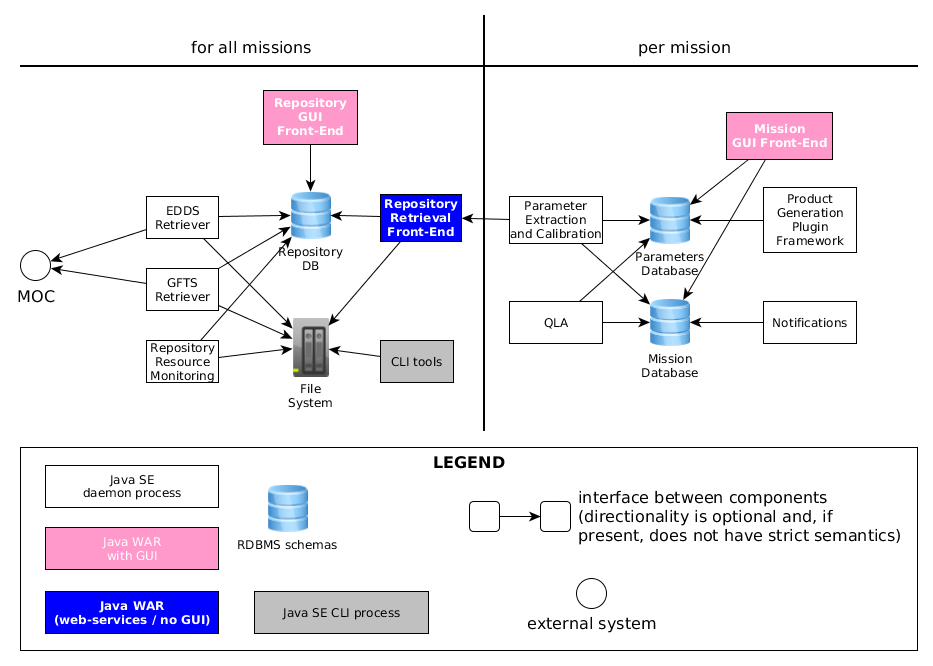
\includegraphics[width=0.9\textwidth]{sw-arch.png}
%    }
    \caption{Proposed software architecture}
    \label{fig:sw-arch}
  \end{figure}

  We offer the following qualifications regarding Figure \ref{fig:sw-arch}:
  \begin{enumerate}
  \item the depicted database icons correspond to distinct \gls{rdbms} schemas
    and not necessarily to distinct databases or database servers\footnote{``clusters'' in
      PostgreSQL terminology.}. Moreover, we expect that in the implementation phase
    most of these schemas will be further split into more specialized ones\footnote{It
    is typically, e.g. to have separate schemas for logging/notifications, user management, etc.}.
  \item the \gls{rdbms} titled ``Mission Database'' does not correspond to a \gls{mib}.
  \end{enumerate}

  Figure \ref{fig:sw-arch} suggests a reasonable and well-defined division between the
  \gls{radacer} and the \gls{gedais} subsystems, an issue that has plagued the project since
  its inception. More specifically, we propose that implementation components which will be
  deployed / installed only once for all missions are considered part of the \gls{radacer}
  subsystem. Conversely, components which will be deployed / installed on a per-mission
  basis are deemed to belong to the \gls{gedais} sub-system.

  Since it is possible that the use of the term ``sub-system'' may have project management
  implications and may necessitate a redefinition of milestones or require
  refactoring of already submitted deliverables, we will be using the more innocuous term
  ``area'' instead of ``sub-system'' for the remainder of this document.

  With the above in mind, to more easily recognize and refer to implementation components
  in a semantic way, we propose the following naming convention:
\begin{verbatim}
  area-componentNameInCamelCase-type
\end{verbatim}

With the following controlled values.
\begin{itemize}
\item for the area:
  \begin{itemize}
  \item RAW: for \gls{rawdar}
  \item GED: for \gls{gedais}
  \end{itemize}
\item for the type:
  \begin{itemize}
  \item DMN: for headless \gls{jse} deamon applications that are supposed to be running as deamons (or, e.g. triggered
    by Cron)
  \item CLI: for interactive, console-based \gls{jse} applications that are supposed to be manually invoked and interacted
    with by a user.
  \item WAR: for \gls{jee} \gls{war} artifacts with a graphical user interface
  \item WS: for \gls{jee} \gls{war} artifacts exposing only web services, without a graphical user interface
  \item DB: for \gls{rdbms} schemas
  \end{itemize}
\end{itemize}

As such, Table \ref{tbl:compo-names} shows the formal names of all implementation components
(identified by their ``friendly name''
that appears in Figure \ref{fig:sw-arch}).

\begin{table}
\begin{tabular}{ l | l }
  \hline\hline
  \gls{edds} retriever & RAW-eddsRetr-DMN \\
  \gls{gfts} retriever & RAW-gftsRetr-DMN \\
  Repository Resource Monitoring & RAW-repoResMon-DMN \\
  Repository DB & RAW-repo-DB \\
  Repository Retrieval Front-end & RAW-repoRetrieval-WAR \\
  Repository \gls{gui} Front-end & RAW-repo-GUI \\
  Repository \gls{cli} tools & RAW-repo-CLI \\
  Parameter Extraction and Calibration & GED-paramExtr-DMN \\
  \gls{qla} & GED-qla-DMN \\
  Parameters database & GED-param-DB \\
  Mission database & GED-mission-DB \\
  Mission \gls{gui} front-end & GED-mission-GUI \\
  Product Generation Plugin Framework & GED-product-DMN \\
  Notifications & GED-notif-DMN \\
  \hline\hline
\end{tabular}
\caption{Normative implementation component names.}
\label{tbl:compo-names}
\end{table}

\section{System Concept Component traceability matrices}
We provide below the traceability matrices from the functional components
of \cite{ref:sow} to the implementation components defined in this deliverable.
The below tables are also used to automatically derive the traceability from the fuctional requirements
of \cite{ref:sow} to the implementation components of this deliverable (and vice-versa).

\begin{func2ImplComp}
  {
      "foo" : ["a", "b", "c"],
      "bar" : ["a2", "b2", "c2"]
  }
\end{func2ImplComp}


\begin{longtable}{l | p{10cm}}
  \caption[Feasible triples for a highly variable Grid]{Feasible triples for
    highly variable Grid, MLMMH.}\\
  \textbf{First entry} & \textbf{Second entry} \\
  \hline
  \endfirsthead
  \multicolumn{2}{c}%
              {\tablename\ \thetable\ -- \textit{Continued from previous page}} \\
              \hline
              \textbf{First entry} & \textbf{Second entry} \\
              \hline
              \endhead
              \hline \multicolumn{2}{r}{\textit{Continued on next page}} \\
              \endfoot
              \hline
              \endlastfoot
              \label{grid_mlmmh} \\
              0 & (1, 11, 13725) (1, 12, 10980), (1, 13, 8235), (2, 2, 0), (3, 1, 0) (1, 11, 13725) (1, 12, 10980), (1, 13, 8235), (2, 2, 0), (3, 1, 0) (1, 11, 13725) (1, 12, 10980), (1, 13, 8235), (2, 2, 0), (3, 1, 0) (1, 11, 13725) (1, 12, 10980), (1, 13, 8235), (2, 2, 0), (3, 1, 0) \\
  0 & (1, 11, 13725) (1, 12, 10980), (1, 13, 8235), (2, 2, 0), (3, 1, 0) \\
  0 & (1, 11, 13725) (1, 12, 10980), (1, 13, 8235), (2, 2, 0), (3, 1, 0) \\
  0 & (1, 11, 13725) (1, 12, 10980), (1, 13, 8235), (2, 2, 0), (3, 1, 0) (1, 11, 13725) (1, 12, 10980), (1, 13, 8235), (2, 2, 0), (3, 1, 0) (1, 11, 13725) (1, 12, 10980), (1, 13, 8235), (2, 2, 0), (3, 1, 0) (1, 11, 13725) (1, 12, 10980), (1, 13, 8235), (2, 2, 0), (3, 1, 0) \\
  0 & (1, 11, 13725) (1, 12, 10980), (1, 13, 8235), (2, 2, 0), (3, 1, 0) \\
  0 & (1, 11, 13725) (1, 12, 10980), (1, 13, 8235), (2, 2, 0), (3, 1, 0) \\
  0 & (1, 11, 13725) (1, 12, 10980), (1, 13, 8235), (2, 2, 0), (3, 1, 0) (1, 11, 13725) (1, 12, 10980), (1, 13, 8235), (2, 2, 0), (3, 1, 0) (1, 11, 13725) (1, 12, 10980), (1, 13, 8235), (2, 2, 0), (3, 1, 0) (1, 11, 13725) (1, 12, 10980), (1, 13, 8235), (2, 2, 0), (3, 1, 0) \\
  0 & (1, 11, 13725) (1, 12, 10980), (1, 13, 8235), (2, 2, 0), (3, 1, 0) \\
  0 & (1, 11, 13725) (1, 12, 10980), (1, 13, 8235), (2, 2, 0), (3, 1, 0) \\
  0 & (1, 11, 13725) (1, 12, 10980), (1, 13, 8235), (2, 2, 0), (3, 1, 0) (1, 11, 13725) (1, 12, 10980), (1, 13, 8235), (2, 2, 0), (3, 1, 0) (1, 11, 13725) (1, 12, 10980), (1, 13, 8235), (2, 2, 0), (3, 1, 0) (1, 11, 13725) (1, 12, 10980), (1, 13, 8235), (2, 2, 0), (3, 1, 0) \\
  0 & (1, 11, 13725) (1, 12, 10980), (1, 13, 8235), (2, 2, 0), (3, 1, 0) \\
  0 & (1, 11, 13725) (1, 12, 10980), (1, 13, 8235), (2, 2, 0), (3, 1, 0) \\
    0 & (1, 11, 13725) (1, 12, 10980), (1, 13, 8235), (2, 2, 0), (3, 1, 0) (1, 11, 13725) (1, 12, 10980), (1, 13, 8235), (2, 2, 0), (3, 1, 0) (1, 11, 13725) (1, 12, 10980), (1, 13, 8235), (2, 2, 0), (3, 1, 0) (1, 11, 13725) (1, 12, 10980), (1, 13, 8235), (2, 2, 0), (3, 1, 0) \\
  0 & (1, 11, 13725) (1, 12, 10980), (1, 13, 8235), (2, 2, 0), (3, 1, 0) \\
  0 & (1, 11, 13725) (1, 12, 10980), (1, 13, 8235), (2, 2, 0), (3, 1, 0) \\
  0 & (1, 11, 13725) (1, 12, 10980), (1, 13, 8235), (2, 2, 0), (3, 1, 0) (1, 11, 13725) (1, 12, 10980), (1, 13, 8235), (2, 2, 0), (3, 1, 0) (1, 11, 13725) (1, 12, 10980), (1, 13, 8235), (2, 2, 0), (3, 1, 0) (1, 11, 13725) (1, 12, 10980), (1, 13, 8235), (2, 2, 0), (3, 1, 0) \\
  0 & (1, 11, 13725) (1, 12, 10980), (1, 13, 8235), (2, 2, 0), (3, 1, 0) \\
  0 & (1, 11, 13725) (1, 12, 10980), (1, 13, 8235), (2, 2, 0), (3, 1, 0) \\
    0 & (1, 11, 13725) (1, 12, 10980), (1, 13, 8235), (2, 2, 0), (3, 1, 0) (1, 11, 13725) (1, 12, 10980), (1, 13, 8235), (2, 2, 0), (3, 1, 0) (1, 11, 13725) (1, 12, 10980), (1, 13, 8235), (2, 2, 0), (3, 1, 0) (1, 11, 13725) (1, 12, 10980), (1, 13, 8235), (2, 2, 0), (3, 1, 0) \\
  0 & (1, 11, 13725) (1, 12, 10980), (1, 13, 8235), (2, 2, 0), (3, 1, 0) \\
  0 & (1, 11, 13725) (1, 12, 10980), (1, 13, 8235), (2, 2, 0), (3, 1, 0) \\
  0 & (1, 11, 13725) (1, 12, 10980), (1, 13, 8235), (2, 2, 0), (3, 1, 0) (1, 11, 13725) (1, 12, 10980), (1, 13, 8235), (2, 2, 0), (3, 1, 0) (1, 11, 13725) (1, 12, 10980), (1, 13, 8235), (2, 2, 0), (3, 1, 0) (1, 11, 13725) (1, 12, 10980), (1, 13, 8235), (2, 2, 0), (3, 1, 0) \\
  0 & (1, 11, 13725) (1, 12, 10980), (1, 13, 8235), (2, 2, 0), (3, 1, 0) \\
  0 & (1, 11, 13725) (1, 12, 10980), (1, 13, 8235), (2, 2, 0), (3, 1, 0) \\
  0 & (1, 11, 13725) (1, 12, 10980), (1, 13, 8235), (2, 2, 0), (3, 1, 0) (1, 11, 13725) (1, 12, 10980), (1, 13, 8235), (2, 2, 0), (3, 1, 0) (1, 11, 13725) (1, 12, 10980), (1, 13, 8235), (2, 2, 0), (3, 1, 0) (1, 11, 13725) (1, 12, 10980), (1, 13, 8235), (2, 2, 0), (3, 1, 0) \\
  0 & (1, 11, 13725) (1, 12, 10980), (1, 13, 8235), (2, 2, 0), (3, 1, 0) \\
  0 & (1, 11, 13725) (1, 12, 10980), (1, 13, 8235), (2, 2, 0), (3, 1, 0) \\
  0 & (1, 11, 13725) (1, 12, 10980), (1, 13, 8235), (2, 2, 0), (3, 1, 0) (1, 11, 13725) (1, 12, 10980), (1, 13, 8235), (2, 2, 0), (3, 1, 0) (1, 11, 13725) (1, 12, 10980), (1, 13, 8235), (2, 2, 0), (3, 1, 0) (1, 11, 13725) (1, 12, 10980), (1, 13, 8235), (2, 2, 0), (3, 1, 0) \\
  0 & (1, 11, 13725) (1, 12, 10980), (1, 13, 8235), (2, 2, 0), (3, 1, 0) \\
  0 & (1, 11, 13725) (1, 12, 10980), (1, 13, 8235), (2, 2, 0), (3, 1, 0) \\    
\end{longtable}
  
\section{Interfaces Context}
\section{Deployment}
\section{Memory and CPU budget}

\begin{comment}



  \begin{mdframed}[style=MyFrame2]
    \begin{enumerate}[label=\alph*.]
    \item The \gls{sdd} shall identify all the external interfaces or refer to the \gls{icd}.
    \item The description in \textless4.4\textgreater, should be based on system block diagram or
      context diagram to illustrate the relationship between this system and
      other systems.
    \end{enumerate}
  \end{mdframed}

\end{comment}


\chapter{Software Components Design}
\label{chap:scd}
\section{Overview}
\label{sec:scd:overview}
\section{Components}
\subsection{Component a}
\subsubsection{type}
\subsubsection{dependencies}
\subsubsection{interfaces}
\subsubsection{processing and data}
\chapter{Requirements Traceability}
\label{chap:traceability}


\begin{appendices}
% nada 
\end{appendices}

\begin{thebibliography}{1}
\bibitem{ref:ecss-e40} \gls{ecss}, ECSS-E-ST-40 Working Group, {\em Space Engineering: Software} ECSS-E-ST-40C, 6 March 2009
\bibitem{ref:sow}ESAC {\em Science Raw Data Archive and Data Ingestion System Statement of Work}, reference ESA-SRE-RAWDAR-SOW-0001, Issue:1, Revision:0, Date of Issue 10/06/2014
\bibitem{ref:sdp}{\em System Development Plan for RAWDAR} --- this document unifies the system development plan for \gls{radacer} and the system development plan
  for GEDAIS (respectively identified as \texttt{ESA-SRE-RADACER-SCP-0001} and \texttt{ESA-SRE-GEDAIS-SDP-0001} in Section 6.1 of \cite{ref:sow}.
\bibitem{ref:sc}{\em RAWDAR System Concept}, Neuropublic, December 2015 (in the context of this project)
for GEDAIS (respectively identified as \texttt{ESA-SRE-RADACER-SCP-0001} and \texttt{ESA-SRE-GEDAIS-SDP-0001} in Section 6.1 of \cite{ref:sow}.  
%\bibitem{ref:esa-telemetry}ESA Packet Telemetry Standard, ESA-PSS-04-106 Issue 1, Jan. 1988
%\bibitem{ref:sample-reports}Email by Laurence O'Rourke to Menelaus Perdikeas (copying Marco Freschi and Vicente Navarro) on July 7th 2015.
%\bibitem{ref:rosetta-mars-express-generic-tmtc}Rosetta / Mars Express Generic TM/TC Interface Control Document, RO-MMT-IF-2011, Issue 2, Revision 2, 30/08/2001.
%\bibitem{ref:ecss-concepts}ECSS-E-70-41A: Ground systems and operations\hairspace{}---\hairspace{}Telemetry
and telecommand packet utilization.
%\bibitem{ref:edds-euicd}EGOS Data Dissemination System\hairspace{}---\hairspace{}External User Interface Control Document (EUICD), Version 7.0, Date 2014-12-17, Reference: EGOS-GEN-EDDS-ICD-1001
and telecommand packet utilization.
%\bibitem{ref:radacer-tn}\gls{radacer} Technical Note, Date 2015-11-23
and telecommand packet utilization.
%\bibitem{ref:oaipmh}{\em The Open Archives Initiative Protocol for Metadata Harvesting}\hairspace{}---\hairspace{}Protocol Version 2.0 of 2002-06-14: \url{http://www.openarchives.org/OAI/2.0/openarchivesprotocol.htm}
%\bibitem{ref:psa}{\em Planetary Science Archive}\hairspace{}---\hairspace{}ESA\'s science data archive for planetary exploration missions \url{http://www.rssd.esa.int/index.php?\project=PSA} % dreadfull ``Undefined control sequence'' bug that took me half a day to debug
%\bibitem{ref:psa}{\em Planetary Science Archive}\hairspace{}---\hairspace{}ESA\'s science data archive for planetary exploration missions \url{http://www.rssd.esa.int/index.php?project=PSA} 
%\bibitem{ref:zabbix}{\em Zabbix, an enterprise monitoring solution} \url{www.zabbix.com}
%\bibitem{ref:scr-meeting}{\em System Concept Review}\hairspace{}---\hairspace{}comments and feedback during the System Concept Review meetings held in December 2015
%\bibitem{ref:soap-ws}{\em soap-ws} Java library, based on Spring-WS, that enables handling SOAP on a purely XML level
  \url{https://github.com/reficio/soap-ws}
%\bibitem{ref:email-2015-12-23-av}Email by Antonio Villacorta 2015-12-23 to Menelaus Perdikeas, Vicente Navarro et al.
\end{thebibliography}
\end{document}
